
\documentclass[12pt,a4paper ]{report}
%\usepackage{paquets}
\usepackage[utf8]{inputenc}
\usepackage[francais]{babel}
\usepackage[T1]{fontenc}
\usepackage{amsmath}
\usepackage{amsthm}
\usepackage{algorithm}
\usepackage{algorithmicx}
\usepackage{listings}
\usepackage{algpseudocode}
%\newtheorem{theorem}{Théorème}
\usepackage[usenames,dvipsnames]{color}
\usepackage{amsfonts}
\usepackage{amssymb}
\usepackage{overpic}
\usepackage{fancybox}
\usepackage{here}
\usepackage{setspace}
\usepackage{colortbl}
\usepackage{multirow}
\usepackage{epsfig}
\usepackage{color}
\usepackage{graphicx}
\usepackage[left=2cm,right=2cm,top=3cm,bottom=3cm]{geometry}
\usepackage[Glenn]{fncychap} %Sonny, Lenny, Glenn, Conny, Rejne, Bjarne, Bjornstrup
\usepackage{fancyhdr}
\usepackage{lettrine}
\newtheorem{montheorem}{Théorème}[chapter]
\newtheorem{maproposition}{Proposition}[chapter]
\newtheorem{madefinition}{Définition}[chapter]
\newtheorem{manotation}{Notation}[chapter]
\newtheorem{moncorollary}{Corollaire}[chapter]
\newtheorem{monlemma}{Lemme}[chapter]
\newtheorem{monexp}{Exemple}[chapter]
\title{Étude des mécanismes de reprise après panne sous ordonnancements équitables $(PD^{2})$}
\author{Diallo Mamadou Gando}
\date{25 juin 2014}


\begin{document}
%\maketitle
\onehalfspacing
\pagestyle{fancy}
%\renewcommand\headrulewidth{1pt}
%\fancyhead[L]{Projet de fin d'étude}
%\fancyhead[R]{Laboratoire d'informatique et d'automatique pour les systèmes }
%\fancyfoot[L]{Diallo Mamadou Gando}
%\fancyfoot[R]{\today}
\fancyhead{} \fancyhead[LO]{\footnotesize \sffamily \nouppercase{\leftmark}}
\fancyhead[CO]{} \fancyhead[RO,LE]{ } \fancyhead[RE]{\footnotesize \sffamily\nouppercase{\rightmark}} \fancyhead[CE]{}
%% pied de page
\fancyfoot[LO]{\footnotesize \it Mise au point d'un algorithme de recherche des services Clouds bas\'ee sur le calcul de similarit\'e}
\fancyfoot[RE]{\small \it Baccar & Boukthir} \fancyfoot[RO,LE]{\thepage}
\fancyfoot[CO]{} \fancyfoot[CE]{}
\renewcommand{\headrulewidth}{0.9pt}
%-------------------------------------------------------------------
\newtheorem{rem}{\bf Remarque}
\newtheorem{hyp}{\bf Hypothèse}
\newtheorem{definition}{\bf Définition}
\newtheorem{proposition}{\bf Proposition}
\newtheorem{lem}{\bf Lemme}
%------------------- Definition de nouvelles commandes ----------------
\def\rref#1{{\rm (\ref{#1})}}
\newcommand\mR{\mathbb{R}}
\newcommand{\defeq}{:=}
\newcommand{\mat}[1]{\begin{pmatrix}
#1
\end{pmatrix}}
%% pied de page

%remerciement

% la structuration d'un document
%\thispagestyle{empty}
%\begin{titlepage}
%\begin{center}
%Manuscrit de these \\
%{{\bf Spécialité : " Automatique et Robotique"}}
%\\ \ \\ Préparée au Laboratoire d'Informatique
%de Robotique et de Microelectronics de Montpellier
%\\ \ \\ Presentee et soutenue publiquement\\ \ \\
%par \\ \ \\ {S. DUPONT}
%\\ \
%\\{le 20 Avril 2001}
%\\ \ \\{\LARGE \hrule \ \\ \bf
%Recherche de sous-structures arborescentes frequentes avec des contraintes d'inclusion floue
%\\ [3mm] \hrule} \ \\ \ \\
%{\bf Directeur de these :} aaaaaaaa rrrrrrrrrr\\
%{\bf Co-Encadrant :} aaaaaaaaaa wwwwwwwww
%\end{center}
%\end{titlepage}
\thispagestyle{empty}
\begin{center}
Ministère de l'Enseignement Supérieur et de la Recherche Scientifique\\
Université de Tunis El Manar \\
Département Informatique \vskip 0.4cm

			
\includegraphics[width=5cm]{en}

%\ \\[-1.3cm]
%\vskip -1.2cm
\Large{\textbf{Projet de Fin d'Année}}

 \vskip -1mm
 présenté par :
 \vskip -0.4mm
 \Large \textbf{Baccar Houssem}
 \vskip -1mm
 \Large \textbf{Boukthir Aymen}
 \vskip 4mm

%\centerline{\footnotesize{de} \small{\textbf{l'Ecole Nationale d'Ing\'enieurs de Tunis}}}
\vskip 1cm

\fbox{
	\begin{minipage}{17cm}
\vspace{0.5cm}
\begin{center}
{\LARGE  {\textbf {\textit  Mise au point d'un algorithme de recherche des services Clouds bas\'ee sur le calcul de similarit\'e }}}
 \vskip 0.2cm
% {\LARGE  { \textbf{\textit{  }}}}
\end{center}
\vspace{0.1cm}
\end{minipage}
}

\vskip 1cm

\vskip 1cm
Encadré par:\\
Mme. Zohra Sbaai \\
Mme. Rawand Guerfel\\
\end{center}
 %\hspace{7cm} Encadré par:

%\begin{tabular}{p{0.5cm}p{2.5cm}p{11cm}}
%
%& ~~ &  \qquad \qquad Mr. Sadok Ben Yahia (FST)\\
%& ~~ &  \qquad \qquad Mr. Ladjel Bellatreche (LIAS)\\
%
%\end{tabular}

\vskip 1cm
\centerline {Année universitaire : 2014-2015}
%\begin{center}
%\centerline{Année universitaire : 2013-2014}
%\end{center}
%\frontmatter 
\pagenumbering{roman}
\chapter*{Remerciements}
\markboth{Remerciements}{}
%\begin{center}\textbf{\Huge \bf {Remerciements}}\end{center}

    Avant de pouvoir élaborer sur le quoi et le comment du projet, nous tenons tout d’abord à exprimer nos remerciements et notre gratitude envers nos encadrantes à L’Ecole Nationale des Ingénieurs de Tunis  \textbf{Mme SBAI Zohra} et \textbf{Mme GUERFEL Rawand} pour leurs conseils, leur savoir-faire, leur expérience et leur le soutien inconditionnel qui nous a permis de franchir bien des obstacles tout au long de la réalisation de ce projet.\\
    Nous tenons aussi à remercier les membres du Jury qui nous font l’honneur de participer à la soutenance et d’évaluer notre travail ainsi que toute personne qui nous a appuyés lors de la réalisation du projet.

%\hspace{13cm}\textbf{Sarar Hammar}






\chapter*{Résumé}
Dû à l'augmentation des nombres de services Cloud et de l'apparition et prolifération du principe de web sémantique , il est devenu indispensable aux utilisateurs  d'avoir à disposition  un moteur de recherche permettant de trouver les services Cloud dont ils ont besoin.
C'est dans ce cadre que s'inscrit notre projet de fin d'année puisque l'objectif principal est de mettre au point un algorithme de recherche des services Clouds qui se base sur la notion de similarité .
L'ontologie du Cloud se reposant sur un ensemble de concepts liés entre eux et pour pouvoir optimiser le résultat du calcul de similarité et ainsi de la recherche des services Cloud, nous nous sommes reposés sur l'implémentation de trois type de similarités : Similarité de concepts , similarité de la propriété objet et la similarité de la propriété de type de donnée.
Et cela pour aboutir à une recherche poussée , précise et adaptée aux services Cloud.
\textbf{Mots Clefs : }Cloud , Ontologie , Similarité , Recherche , Algorithme\\ \ \\

\chapter*{Abstract}
Due to increasing number of Cloud services and the emergence and proliferation of semantic web, it has become essential for users to have access to  a search engine that can find the cloud services suitable to their needs .
This  fits our year-end project perfectly since the main objective is to develop a search algorithm for Clouds of services which is based on the concept of similarity .
The ontology of cloud resting on a set of interrelated concepts and in order to optimize the calculation result of similarity  cloud services  search results , we agreed on implementing three types of similarities : Similarity concepts, similarity of the object property and the similarity of the data type property.
And the purpose is to achieve and extensive , accurate and suitable search  for cloud services .
\textbf{Keywords :} Cloud, Ontology , Similarity , Research , Algorithm.\\ \ \\
%\chapter*{Dédicace}
\markboth{Dédicace}{}
%\begin{center}\textbf{\Huge \bf {Dédicace}}\end{center}

\hspace{2cm}
\hspace{2cm}

\hspace{2cm}
\hspace{2cm}

Qu’il me soit permis à travers ce modeste projet de fin d’études en vue de l’obtention du diplôme d’ingénieur en informatique d’exprimer ma plus profonde reconnaissance à : \\

Mes parents Mohamed Habib Hammar \& Saloua Ben Dhia : Que nulle dédicace ne puisse exprimer ce que je leur dois, pour leur bienveillance depuis ma plus jeune enfance et leur affection. Ceux qui ont sacrifié leurs plus belles années pour embellir les miennes, ceux à qui je dois ma réussite, aucun mot ne serait assez pour témoigner la sincérité des sentiments que j’éprouve à leur égard. \\

Ma grande sœur \textbf{Roua} et mon petit frère \textbf{Mohamed} : Qui n’ont jamais cessé de me soutenir, m’assister et m’encourager. Ce travail est en témoignage de mon profond amour et ma gratitude envers eux.\\

La mémoire de mes grands-pères \textbf{Mohamed Hammar} \& \textbf{Habib Ben Dhia}.\\

Tous mes amis spécialement \textbf{Amine}, \textbf{Meriam} \& \textbf{Salma}.\\

Tous les membres de ma famille.\\

Je leur dédie ce modeste travail en témoignage de mon profond dévouement et ma gratitude infinie pour tous les efforts qu'ils ne cessent de me fournir.\\ \ \\



\hspace{15cm}\textbf{Sarar} 
\chapter*{Glossaire}
\markboth{Glossaire}{}
\textbf{OWL} : Ontology web language
\tableofcontents
%\addcontentsline{toc}{chapter}{Introduction Générale}
\listoftables
\listoffigures
\newpage %\thispagestyle{empty} \vspace*{5mm} \newpage
\pagenumbering{arabic}
%--------------------------------------
%\addcontentsline{toc}{chapter}{Remerciement}
\addcontentsline{toc}{chapter}{Introduction Générale}
\chapter*{Introduction Générale}
\markboth{Introduction Générale}{}

    \hspace{1.5cm} \textbf{ Contexte et problématique du travail}

        Le "Cloud Computing" ou "L'Informatique en Nuage" peut-être définie comme un paradigme informatique distribué à grande échelle dans lequel on trouve une collection de plateformes, puissance de calcul , espaces de stockages et autres services qui sont dynamiquement évolutifs,virtualisés et qui sont délivrés aux clients à travers Internet.\\
        Cependant, il n'y a pas de standards et de protocoles pour gérer la recherche des différents Clouds d'où la nécessité d'avoir un engin de recherche pour les services Cloud.\\
        Pour augmenter nos chances de découvrir les services clouds appropriés, nous avons besoin de représenter les relations sémantiques entre les différents les concepts du Cloud service en ayant recours à une ontologie du Cloud.\\
        Cette Ontologie nous permettra de  raisonner sur la similarité entre les concepts du Cloud et aboutir à un mécanisme efficace pour la recherche des services Clouds.\\

    \hspace{1.5cm} \textbf{ Contributions  }\\
        Notre projet consiste en la réalisation d'une application java , qui permet de raisonner sur le language OWL (Ontologie Web Language) à travers un algorithme de recherche basé sur le calcul de la similarité entre les différents individus d'une ontologie et ainsi de faciliter la recherche des services Cloud sur le Web en permettant aux utilisateurs de trouver un service Cloud spécifique ou de trouver un service qui est similaire à la requête de l'utilisateur en se basant sur le résultat de la similarité.\\




    \hspace{1.5cm} \textbf{ Organisation du projet }\\
    L’organisation de notre rapport se présente comme suit :\\Dans le premier chapitre, nous allons aborder les définitions des concepts ayant une importance relative à la réalisation du projet  tel que : Le Cloud computing son architecture et ses différentes couches, l’ontologie et les environnements de developpement qui la permettent sa construction, l'OWL, La similarité etc.\\
    Dans le deuxième chapitre  nous allons nous intéresser de plus près à la similarité sur ses trois formes (sur les concepts, sur les propriétés d'objets et sur les propriétés de données) : Leurs formules de calcul et leur complexité algorithmique.\\
    Dans le troisième chapitre  nous allons aborder les étapes d'implémentation de notre projet (Conception, réalisation, test et validations...) et les outils techniques utilisés à cette fin.\\
    Nous concluons ce rapport par un bilan général sur nos contributions et nos constations, et la discussion  des perspectives qui en dérivent.\

\chapter{\'{E}TAT DE L’ART} \label{intro}
%------------------------------------------
\section{Introduction}
    Dans ce chapitre nous allons présenter un état de l’art sur le Cloud Computing.
    Nous commencerons  en premier temps par introduire le concept de Cloud Computing.
    Suite à cela nous aborderons les différentes couches qui constituent le Cloud.
    Ensuite nous présenterons les différents types de déploiements du Cloud.
    Enfin nous allons terminer par définir ce qu’est une ontologie et l’avantage d’avoir recours à une ontologie du Cloud dans le mécanisme de recherche.

\section{Concepts Fondamentaux}
    \subsection{Cloud Computing}
        \subsubsection{1.2.1.1 Définition et apport}


                Le Cloud computing repose sur le partage des ressources pour atteindre la cohérence et les économies d'échelle, semblable à un utilitaire (comme le réseau d'électricité) sur un réseau .Il est à la base  d’une large infrastructure convergée et partagé de services.\\

                Cloud computing, ou également appellé "le nuage informatique", met également l'accent sur la maximisation de l'efficacité des ressources partagées. Les nuages de ressources sont généralement non seulement partagé par plusieurs utilisateurs, mais sont également réaffectées dynamiquement selon la demande. Par exemple, un centre informatique en nuage qui sert les utilisateurs européens pendant les heures d'affaires avec une application spécifique (par exemple, e-mail) peut réaffecter les mêmes ressources pour servir les utilisateurs d'Amérique du Nord avec une autre application (par exemple, un serveur Web) . Cette approche devrait permettre de maximiser l'utilisation de la puissance de calcul en réduisant ainsi les dommages environnementaux ainsi  que la dépense  d'énergie, climatisation, etc…  Avec le cloud computing, plusieurs utilisateurs peuvent accéder à un seul serveur pour récupérer et mettre à jour leurs données sans avoir à acheter des licences pour des applications différentes.\\

                Il est le résultat de l'évolution et l'adoption de technologies et des paradigmes existants. Son objectif est de permettre aux utilisateurs de tirer profit de l'ensemble de ces technologies, sans avoir besoin de connaissances approfondies dans le  sujet ou de l'expertise avec chacun d'entre eux. Le nuage a pour objectif de réduire les coûts, et aide les utilisateurs à se concentrer sur leur cœur de métier plutôt que d'être entravé par des obstacles informatiques. \\

                La principale technologie habilitante pour le cloud computing est la virtualisation. Les logiciels de virtualisation séparent un dispositif informatique physique dans un ou plusieurs dispositifs «virtuels», chacun pouvant être facilement utilisé et géré pour effectuer des tâches informatiques. La virtualisation au niveau du système d'exploitation permet la création d’un système évolutif qui optimise l’allocation des ressources inactives et ainsi améliore drastiquement la performance et l’économie d’énergie. La virtualisation offre l'agilité nécessaire pour accélérer les opérations informatiques, et réduit le coût en augmentant l'utilisation de l'infrastructure.\\
                L’Informatique autonome permet d’automatiser le processus par lequel les ressources utilisateurs sont approvisionnés. En minimisant la participation des utilisateurs, l’automatisation accélère le processus, réduit les coûts de main-d'œuvre et réduit la possibilité d'erreurs humaines.\\


                Le Cloud computing adopte des concepts de l'architecture orientée services SOA qui peuvent aider l'utilisateur à briser ces problèmes dans des services qui peuvent être intégrés pour fournir une solution. Il fournit toutes ces ressources comme des services, et fait usage des normes bien établies et des meilleures pratiques acquises dans le domaine de l'architecture SOA pour permettre un accès mondial et facile aux services du cloud computing de manière standardisée.

                Le Cloud computing exploite également des concepts de l'informatique utilitaire afin de fournir des données pour les services utilisés. Ces mesures sont à la base des modèles Cloud public pay-per-use. En outre, les services mesurés sont une partie essentielle de la boucle de rétroaction dans l'informatique autonome, permettant des services à l'échelle, à la demande pouvant être récupérés en cas de panne  automatique .\\

                C'est une sorte de grille de calcul qui  a évolué en abordant la QoS (qualité de service) et des problèmes de fiabilité. Et fournit les outils et les technologies pour construire des données / calculer  des applications parallèles intensives avec des prix beaucoup plus abordables par rapport aux techniques traditionnelles de calcul parallèle.\\

                Le Cloud computing partage des caractéristiques avec:
            \begin{itemize}
                \item[\quad $\bullet$]Modèle client-serveur :client-serveur informatique se réfère largement à toute application distribuée qui distingue entre les prestataires de services (serveurs) et les demandeurs de services (clients).
                \item[\quad $\bullet$]Grid computing : Une forme de calcul distribué et parallèle, par laquelle un« super-ordinateur et virtuel »est composé d'un groupe d'ordinateurs en réseau, faiblement couplés agissant pour réaliser de très grandes tâches.
                \item[\quad $\bullet$]Mainframe informatique : ordinateurs puissants utilisés principalement par les grandes organisations pour les applications critiques, généralement des données en vrac de traitement tels que: recensement; statistiques de l'industrie et de la consommation; la police et les services secrets de renseignement; progiciel de gestion intégré et traitement des transactions financières.
                \item[\quad $\bullet$]L'informatique utilitaire : Emballages de ressources informatiques, tels que calcul et de stockage, comme un service mesurée semblable à un service public traditionnel, comme l'électricité.
                \item[\quad $\bullet$]Peer-to-peer - Une architecture distribuée sans la nécessité d'une coordination centrale. Les participants sont à la fois les fournisseurs et les consommateurs des ressources (en contraste avec le modèle client-serveur traditionnelle).
            \end{itemize}
            Cloud computing présente les principales caractéristiques suivantes:\\
            \begin{itemize}
                \item[\quad $\bullet$]Une grande Agilité qui améliore la capacité des utilisateurs à redistribuer les ressources d'infrastructure technologique.\\
                \item[\quad $\bullet$]L'indépendance des dispositifs et des emplacements  permettent aux utilisateurs d'accéder à des systèmes utilisant un navigateur web indépendamment de leur emplacement ou de ce dispositif qu'ils utilisent (par exemple, PC, téléphone mobile). Comme l'infrastructure est hors site (généralement fournie par un tiers) et accessible via Internet, les utilisateurs peuvent se connecter à partir de n'importe où.
                \item[\quad $\bullet$]La maintenance des applications de cloud computing est plus facile, parce qu'ils ne doivent pas nécessairement être installés sur l'ordinateur de chaque utilisateur et peuvent être accessibles à partir de différents endroits.
                \item[\quad $\bullet$]Permet le partage des ressources et des coûts à travers une grande bibliothèque d'utilisateurs permettant ainsi la centralisation de l'infrastructure dans des endroits avec des coûts inférieurs (tels que l'immobilier, l'électricité, etc.)
                \item[\quad $\bullet$]Fiabilité améliorée avec l'utilisation de plusieurs sites redondants, ce qui rend la conception du cloud computing approprié pour la continuité d'activité.
                \item[\quad $\bullet$]Évolutivité et l'élasticité ("à la demande") via le provisionnement des ressources sur une base libre-service  en temps quasi-réel.
            \end{itemize}
            La sécurité peut être améliorée grâce à la centralisation des données, les ressources axées sur la sécurité accrues, etc., mais des inquiétudes persistent à propos de  perte de contrôle sur certaines données sensibles, et le manque de sécurité pour les noyaux stockées. La sécurité est souvent  meilleure que dans les autres systèmes traditionnels, en partie parce que les fournisseurs sont en mesure de consacrer des ressources à la résolution des problèmes de sécurité que de nombreux clients ne peuvent pas se permettre de les voir attaqués.  Cependant, la complexité de la sécurité est considérablement augmentée lorsque les données sont distribuées sur une zone plus large ou sur un plus grand nombre d'appareils, ainsi que dans les systèmes multi-locataires partagés par les utilisateurs indépendants. En outre, l'accès des utilisateurs à des journaux d'audit de sécurité est impossible. Les installations de cloud privé sont en partie dirigées par le désir des utilisateurs à conserver le contrôle de l'infrastructure et d'éviter de perdre le contrôle de la sécurité de l'information.
                \subsubsection{1.2.1.2 Architecture du Cloud}
            Dans ce modèle, il ya trois couches de services différents qui sont utilisés pour spécifier ce qui est provisionné, Infrastructure as a Service (IaaS), Platform as a Service (PaaS) et Software as a Service (SaaS). En outre, il ya trois autres couches qui ne sont pas fournis comme services aux usagers. \\
            \begin{figure}[H]
            \centering
            % Requires \usepackage{graphicx}
            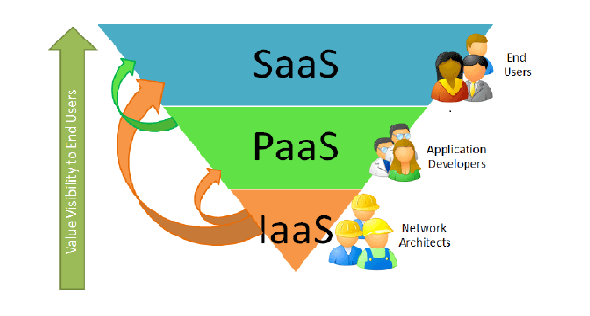
\includegraphics[width=12cm]{trois_couche_cloud}\\
             \caption{les trois couche du Cloud}\label{trois_couche_cloud}
            \end{figure}
        \begin{itemize}
            \item[\quad $\bullet$] Infrastructure as a Service (IaaS):Dans le modèle Cloud de service le plus élémentaire et selon l'IETF (Internet Engineering Task Force), les fournisseurs de IaaS offrent des ordinateurs et d'autres ressources virtuelles aux clients. Une large panoplie  d’hyperviseurs dans le système de soutien Cloud peut supporter un grand nombre de machines virtuelles et la capacité à l'échelle des services de haut en bas selon les différentes exigences des clients.) Les nuages IaaS offrent souvent des ressources supplémentaires comme une bibliothèque de machines virtuelles image disque, le stockage de bloc brut, et le fichier ou un objet de stockage, les pare-feu, les équilibreurs de charge, les adresses IP , les réseaux locaux virtuels (VLAN), des faisceaux de logiciels. Les fournisseurs IaaS-cloud fournissent ces ressources à la demande depuis leurs grandes piscines installées dans les centres de données. Pour la connectivité large zone, les clients peuvent utiliser l'Internet ou les nuages porteurs (réseaux privés virtuels dédiés).

                Pour déployer leurs applications, les utilisateurs de Cloud peuvent installer les systèmes d'exploitation de leur choix et leurs logiciels d'application sur l'infrastructure Cloud. Dans ce modèle, les correctifs et les utilisateurs de Cloud maintiennent les systèmes d'exploitation et le logiciel d'application. Les fournisseurs de Cloud facturent généralement des services IaaS sur une base informatique utilitaire: le coût reflète la quantité des ressources allouées et consommés.



                \item[\quad $\bullet$] Platform as a Service (PaaS):
                Dans les modèles PaaS, les fournisseurs de Cloud offrent une plate-forme informatique, comprenant typiquement un système d'exploitation, l'environnement d'exécution du langage de programmation, base de données, et le serveur web. Les développeurs d'applications peuvent développer et gérer leurs solutions de logiciels sur une plate-forme de Cloud sans le coût et la complexité de l'achat et la gestion des couches matérielles et logicielles sous-jacentes. Le PaaS offre des plateformes comme Microsoft Azure et Google App Engine, les ressources informatiques et de stockage sous-jacents varient automatiquement pour correspondre à la demande d'application de sorte que l'utilisateur du nuage n'a pas à allouer des ressources manuellement. Ce dernier a également été proposé par une architecture visant à faciliter en temps réel dans les environnements de cloud computing. Bien d’autres types d'applications encore plus précis peuvent être fournis par l'intermédiaire de PaaS.
.
                \item[\quad $\bullet$] Software as a Service (SaaS):
                Dans le modèle d'affaires en utilisant un logiciel comme un service (SaaS), les utilisateurs bénéficient d'un accès aux logiciels d'application et des bases de données. Les fournisseurs de Cloud gérent l'infrastructure et les plates-formes qui exécutent les applications. SaaS est parfois appelé «logiciel à la demande" et est généralement un prix sur une base pay-per-utilisation ou à l'aide d'un abonnement.\\

                Dans le modèle SaaS, les fournisseurs de Cloud installent et utilisent le logiciel d'application dans le nuage et les utilisateurs de Cloud peuvent accéder au logiciel du Cloud clients. Le Nuage d’utilisateurs ne configure  pas l'infrastructure Cloud et de plate-forme où l'application fonctionne. Ceci élimine le besoin d'installer et d'exécuter l'application sur des ordinateurs de l'utilisateur de nuages, ce qui simplifie la maintenance et de soutien. Les applications Cloud sont différentes des autres applications qui peuvent être atteints par clonage de tâches sur plusieurs machines virtuelles au moment de l'exécution pour répondre à la demande changeante de travail et leur évolutivité.. Ce processus est transparent pour l'utilisateur de nuage, qui ne voit qu’un point d'accès unique. Pour accueillir un grand nombre d'utilisateurs de Cloud computing, les applications Cloud peuvent être mutualisées, c’est à dire que toute machine sert plus d'une organisation de l'utilisateur de nuage.\\

                Le modèle de tarification pour les applications SaaS est généralement un abonnement mensuel ou annuel forfaitaire par utilisateur,  donc le prix est extensible et ajustable si les utilisateurs sont ajoutés ou supprimés à tout moment.\\

                Ses partisans affirment que le  SaaS permet à une entreprise la possibilité de réduire les coûts d'exploitation IT par l'externalisation de la maintenance matérielle et logicielle et le soutien au fournisseur de cloud. Cela permet à l'entreprise de réaffecter les opérations informatiques qui coûte plus de dépenses de matériel / logiciel et les charges de personnel, en vue d'atteindre d'autres objectifs. En outre, avec des applications hébergées au centre, des mises à jour peuvent être effectuées sans la nécessité pour les utilisateurs d'installer un nouveau logiciel. Un inconvénient de SaaS est que les données des utilisateurs sont stockées sur le serveur du fournisseur de Cloud. En conséquence, il pourrait y avoir un accès non autorisé aux données. Pour cette raison, les utilisateurs sont de plus en plus pour l'adoption de systèmes intelligents de gestion de clés tiers pour aider à sécuriser leurs données.\\
            \end{itemize}
        \subsubsection{1.2.1.3Types de Déploiment}
            on distingue trois type de déploiment de cloud selon l'emplacement des ressources physiques qui fournissent les services:
                \begin{itemize}
                    \item[\quad $\bullet$]Le Cloud privé:\\
                    Le cloud privé est un type de cloud computing qui offre des avantages similaires à cloud public, y compris l'évolutivité et en libre-service, mais à travers une architecture propriétaire. Contrairement à des clouds publics, qui fournissent des services à de multiples organisations, un cloud privé est dédié à une seule organisation.
                    \item[\quad $\bullet$]Le cloud public:\\
                    Un cloud public est fondée sur le modèle de cloud computing standard, dans lequel un prestataire de services fait des ressources, telles que les applications et le stockage, à la disposition du grand public sur Internet. Services de cloud publics peuvent être libres ou offerts sur un modèle pay-per-utilisation.
                    \item[\quad $\bullet$]Le Cloud hybride:\\
                    Cloud hybride est un environnement de cloud computing qui utilise un mélange de sur site, cloud privé et des services de cloud public à l'orchestration entre les deux plates-formes. En permettant à des charges de travail de se déplacer entre les nuages privés et publics comme les besoins informatiques et les coûts changent, cloud hybride donne aux entreprises une plus grande flexibilité et plus d'options de déploiement de données.

                \end{itemize}
                    \begin{figure}[H]
                    \centering
                    % Requires \usepackage{graphicx}
                    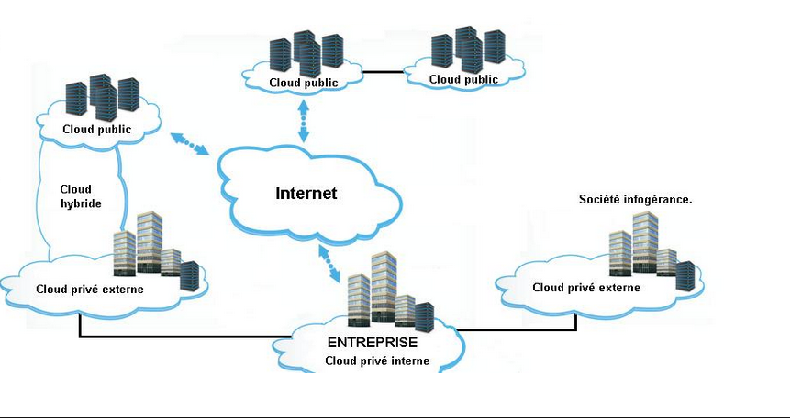
\includegraphics[width=12cm]{cloud_prive_public_hybride}\\
                    \caption{les trois couche du Cloud}\label{cloud_prive_public_hybride}
                \end{figure}
            \subsection{Ontologies}
                \subsubsection{1.2.2.1 Définition}
                     Une ontologie est une spécification explicite d’une conceptualisation d’un domaine[Gruber 1993]\\
                Elle peut fournir un vocabulaire contrôlé de concepts, chacun avec une sémantique qui est explicitement définie et compréhensible par la machine. Elle fournit également une compréhension commune d'un domaine d'intérêt pour soutenir la communication entre les ordinateurs et les humains en définissant des théories de domaine partagées. Dans le domaine de la récupération de l'information, l'ontologie qui se compose d'un ensemble de concepts et de relations entre concepts est utilisé pour traiter les requêtes des utilisateurs.\\
                Avec une ontologie Cloud, nous pouvons développer un système intelligent courtier d'adaptation qui fonctionne sur la base de la compréhension des ressources autres que les noms littéraux. Le système correspondant utilisera les connaissances à partir d'une ontologie pour raisonner sur la mesure de similarité entre les concepts autres que des termes. Dans ce contexte, le principal problème est de construire une ontologie significative dont le raisonnement est approprié pour la découverte des services Cloud. L'architecture et la mise en œuvre de notre système de découverte consiste d'agents utilisateurs, les agents de fournisseurs, et agents de correspondance .Notre approche utilise les avantages du système à base d'agents et le mécanisme d'appariement sémantique en utilisant un nuage ontologie.\\

                \subsubsection{1.2.2.2 Environnements de développement d’ontologie}
                    On trouve plusieurs éditeurs supportant tout le processus de développement des ontologies. Parmis lesquels on cite:\\
                    \begin{itemize}

                        \item[\quad $\bullet$]The Neon Toolkit : c'est un logiciel open source multiplateforme pour le développement d'ontologie. Il est basé sur la plateforme populaire Eclipse et fournit un très grand ensemble de plugins qui couvrent une varieté d'activité. \\
                        \item[\quad $\bullet$]Vitro : c'est un éditeur à usage général d'ontologie du web qui permet de créer et charger des ontologies en format OWL
                        \item[\quad $\bullet$]Protégé sous plusieurs versions qui a été développé dans Standford University\\
                    \end{itemize}
                \subsubsection{1.2.2.3 Langages de développement d’ontologies}
                Il existe plusieurs types de langage de description d'ontologies notamment:
                    \begin{itemize}
                         \item[\quad $\bullet$]Logiques de description:\\
                          langages de représentation de connaissances dont le formalisme s’appuie sur les notions de concepts, de rôles et d’instances

                         \item[\quad $\bullet$]OWL : Ontology Web Language:\\
                          Il est adopté par la recommendation W3C et utilisé comme le principal langage de représentation de connaissances basé sur XML et les logiques de description

                         \item[\quad $\bullet$]RDF: Ressource Description Framework\\
                          Il est basé sur XML et permet de représenter les connaissances sous la forme des triplets, Sujet, Prédicats, Objet

                         \end{itemize}
                \subsubsection{1.2.2.4 OWL}
                    Le langage d'ontologie Web OWL est un langage de balisage sémantique pour l'édition et le partage des ontologies sur le Web. OWL est développé comme une extension de vocabulaire de RDF (Resource Description Framework)
                    \begin{itemize}
                    \item[\quad $\bullet$]Individus : Objets particuliers du domaine
                    \item[\quad $\bullet$]Classe: un groupe d'individus partageant les mêmes caractéristiques. Les classes définies par l'utilisateur sont d'ailleurs toutes des enfants de la  super-classe OWL:Thing.
                    \item[\quad $\bullet$]Propriété : permet de définir des faits ou des relations entre ces classes. OWL fait une distinction entre :
                        \begin{itemize}
                        \item[\quad $\cdot$]Propriétés d'objet: définit une propriété entre deux individus d'une classe ou de plusieurs classes, . Exemple : hasBrother .
                        \item[\quad $\cdot$]Propriétés de données: définit une relation entre une valeur ou donnée et un individu d'une classe. Exemple : hasName.
                        \end{itemize}

                    \end{itemize}
                \section{Recherche basée sur l'ontologie et travaux existants }
                    Les mécanismes de découverte de service Cloud basée sur l'ontologie est devenu un sujet intéressant. De nombreux algorithmes, systèmes et approches ont été proposés pour assurer cette découverte. Nous allons essayer de citer les travaux les plus récents dans cette section.
                    Miranda Zhang et al. [1] ont proposé une ontologie, nommé Cocoon spécifique pour première la couche première, IaaS. Ils ont également proposé un système, CloudRecommender ayant comme objectif principal la découverte de différentes ressources offerts par cette couche. La découverte dans ce travail est limitée à la couche IaaS.
                    Nous citons également le travail de Francesco Moscato et al. [2] qui propose une API pour assurer l'interopérabilité des services multiples offerts par différents Clouds. Cela va assurer une découverte, basée sur l'ontologie, plus précise et plus intelligent.
                    Ces travaux se sont limités à la simple découverte des services Cloud. Cependant, les travaux de Sim et al. [3, 4] et Bhama et al.[5] ont utilisé la similarité dans la recherche des services Cloud. En effet, le travail de Bhama et al.[5] ont visé la nécessité de l’utilisation du raisonnement de similarité dans  la découverte des services Cloud. En effet, ils ont proposé quelques formules nécessaires à utiliser lors du recherche de service Cloud basée sur l’ontologie.
                    Sim et al. [3, 4] ont proposé Cloudle, un moteur  de recherche de service de cloud basé sur l'ontologie. Pour y faire,  Cloudle, cherche les services appropriés dans l’ontologie en utilisant la similarité et les classe selon leurs utilités, leurs prix et leurs disponibilités.
                    C’est  dans ce sens que s’oriente ce PFA. En effet, nous proposons un moteur de recherche de service Cloud basée sur l’ontologie. Plus précisément, et pour offrir à l’utilisateur final le service le plus approprié  à sa demande, nous nous basons sur la similarité des services Cloud qui est classées en trois types principaux à savoir :similarité de concepts, similarité de propriété d’objet et similarité de propriété de données. L’approche est détaillée dans le chapitre suivant.


                \section{Conclusion}

                Ce chapitre a eu pour objectif d’introduire le cadre de l’élaboration de notre projet.
                Nous avons donc présenté le Cloud Computing avec les différentes couches qui le composent et les différents type de Cloud existants et nous avons aussi introduit la notion d’ontologie et expliqué les avantages qui nous ont incités  à choisir de travailler sur l’ontologie du Cloud.

























\chapter{Contribution : Recherche basée sur la similarité} \label{intro}
%------------------------------------------
\section{Introduction}
    La recherche sémantique a pour but de traiter les requêtes de l'utilisateurs selon des liens logiques entre les concepts ou les entités. Il existe plusieurs méthodes et approches avancées pour établir ces liens. Parmis ces méthodes on cite le calcul de la similarité suivant les liens de parneté, les proprietés d'objet et les proprieté de valeurs.
    Pour appliquer le mécanisme de recherche sémantique basé sur la similarité on doit parcourir tout les éléments de l'ontologie et faire les calculs mathématique nécessaires à fin d'optimiser la précision de la recherche.
    Dans ce chapire on va introduitre les trois approches théorique de calcul de la similarité.Ensuite on va présenter les algorithmes permettant d'implémenter ces approches.

\section{Recherche basée sur la similarité}
        Dans la procédure de raisonnement, la similarité entre deux concepts est déterminée en consultant une ontologie du Cloud. Il existe trois méthodes pour la détermination de la similarité qui sont :\\
		Similarité de concepts, Similarité de la proprieté objet et la Similarité de la proprieté type donnée.


    \subsection{Formules mathématiques utilisées}

        \subsubsection{2.2.1.1 similarité de concepts}
            La similarité usuelle trouve seulement  la correspondance basée sur les chaines  de caractères entre les étiquettes alors que la similarité de concepts calcul la similarité entre les concepts qui ont la même signification mais sont exprimés  de façon différente.\\


			$$ sim_{con}(a,b) = | Super(A) \cap Super(B) | / | Super(A) |$$\\

            Où,\\
            A et B sont les concepts des individus a et b respectivement.\\
            Super(A) et Super(B) sont l’ensemble des super concepts qui peuvent être atteints à partir des concepts A et B.\\
            Les étapes de la détermination de la similarité de concepts:
                 \begin{itemize}
                    \item[\quad $\bullet$] 1. Considérer les deux individus « a » et « b » pour lesquels la similarité de concepts doit être calculée.
                    \item[\quad $\bullet$] 2. Compter tous les supers concepts qui peuvent être atteints à partir de chacun des concepts spécifiques « A » et « B » des individus « a » et »b » .
                    \item[\quad $\bullet$] 3. Déterminer les super concepts qui peuvent être atteints à partir de « A » et « B ».
    	           \item[\quad $\bullet$] 4. Diviser le résultat de l’étape 3 par le résultat de l’étape 2 (pour l’individu « a » ).
                 \end{itemize}


    \subsubsection{2.2.1.2 Similarité de propriété objet}
        Les propriétés objets représentent les significations des concepts et fournissent aussi les relations entre les concepts de l’ontologie.\\


        $$ sim_{obj}(a,b)=_{(x,y)\cup}Sim(x,y)/|O(a)|$$\\

        Où,\\
        U={ (x,y) | (a,p,x)   O(a), (b,p,y)     O(b) }\\
        O(a)  est un ensemble de triplets contenant les propriétés objets des individus a et b
        U  est l’ensemble des valeurs d’objets avec le prédicat commun p entre les individus « a » et « b » dans chaque triplet 0(a) et 0(b) .\\

        Les étapes de la détermination de la similarité de la propriété objet:\\
        \begin{itemize}

             \item[\quad $\bullet$]1 Considérer les deux individus « a » et « b » pour lesquels la similarité de concepts doit être calculée.
             \item[\quad $\bullet$]2 Déterminer O(a) et O(b) qui sont les ensembles de triplets contenant les propriétés objets des individus « a » et « b » respectivement.
             \item[\quad $\bullet$]3 Déterminer | O(a) | qui est le nombre d’éléments de l’ensemble O(a).
             \item[\quad $\bullet$]4 Identifier U comme l’ensemble des valeurs d’objets ayant p comme prédicat commun de « a » et « b » dans O(a) et O(b) respectivement.
             \item[\quad $\bullet$]5 Déterminer sim(x,y) pour toutes les valeurs d’objets identifiés dans l’étape 4.
             \item[\quad $\bullet$]6 Faire l’addition de tous les résultats individuels obtenus dans l’étape 5.
             \item[\quad $\bullet$]7 Diviser le résultat de l’étape  6 par le résultat de l’étape 3 (pour l’individu « a »).
          \end{itemize}



    \subsubsection{2.2.1.3 Similarité de proprieté de type de donnée}
        Similarité de la propriété de type de donnée:\\
        Ces propriétés représentent le contexte des concepts et sont aussi des attributs des concepts dans l’ontologie.\\

		$$ sim_{data}(a,b)=_{(x,y,p)\vee}Comp(x,y,p)/|D(a)|$$\\
        Où,\\

		V = {(x,y,p) | (a,p,x)	D(a),(b,p,y) D(b)}\\
		$$ Comp(x,y,p) = 1 - (|x-y|)/ Max_{distance}(x,p)$$
		$$ Max_{distance}(x,p) = max_{ i I(p)}(| x-i |)$$
		$$ I(p) = {i |(s,p,i)  Ontology}$$
		

        D(a) est un ensemble de triplets qui contiennent les propriétés de type de donnée de l’individu « a ».
        V est l’ensemble des valeurs des types de données ayant p comme prédicat commun des individus « a » et « b ».\\

        3.3.1 Les étapes de la détermination de la similarité de la propriété de type de donnée
        \begin{itemize}


	       \item[\quad $\bullet$]1. Considérer les deux individus « a » et « b » dont la similarité de concepts doit être calculée.
            \item[\quad $\bullet$]2. Identifier D(a) et D(b) qui sont les ensembles de triplets contenant les propriétés de type de
 	      donnée des individus « a » et « b » respectivement.
	       \item[\quad $\bullet$]3. Déterminer | O(a) | qui est le nombre des éléments de l’ensemble O(a).
	       \item[\quad $\bullet$]4. Identifier V comme l’ensemble des valeurs d’objets ayant p comme prédicat commun des
     	individus « a » et « b » dans D(a) et D(b) respectivement.
            \item[\quad $\bullet$]5. Déterminer Comp(x,y,p) qui est la similarité entre les valeurs « x » et « y » des type de données sur le prédicat commun p.
            \item[\quad $\bullet$]6. Déterminer la distance maximale qui peut être atteinte en se basant sur la valeur « x ».
            \item[\quad $\bullet$]7. Utiliser le résultat de l’étape 6 et la distance entre « x » et « y » pour déterminer la similarité entre valeurs des types de données de « a » et de « b ».
        \end{itemize}

\subsection{Solution algorithmique proposé}
\subsubsection{2.2.2.1 Similarité de concept}

\begin{algorithm}[H]
\caption{ Calcul la valeur de la similarité de concepts}
%\algsetup{indent=2em}
\begin{algorithmic}[1]
\State Procedure réel conceptSimilarity(Concept A,Concept B)
\State $\{$
\State retourner SuperInterSuper(A,B)/Super(A)
\State  $\}$
\end{algorithmic}
\end{algorithm}

\begin{algorithm}[H]
\caption{ Calcul du nombre de noeuds communs }
%\algsetup{indent=2em}
\begin{algorithmic}[1]
\State Procedure entier SuperInterSuper(Concept A, Concept B)
\State $\{$
\State entier supA=Super(A)
\State entier supB=super(B)
\If{(supA==1 or supB==1)}
\State retourner 1
\EndIf
\If{(supA==supB)}
\If{(A==B)}
\State retourner supA
\EndIf
\ElsIf{(supA>supB)}
\State retourner SuperInterSuper(A->parent,B)
\Else
\State retourner SuperInterSuper(A,B->parent)
\EndIf
\State $\}$
\end{algorithmic}
\end{algorithm}
				
				
        \subsubsection{2.2.2.2 Similarité de propriété d'objet}
		
			\begin{algorithm}[H]
			\caption{ Calcul de la similarité de la propriété objet }
			%\algsetup{indent=2em}
			\begin{algorithmic}[1]
			\State Procedure réel similaritéDePropriétéObjet(Concept A, Concept B)
            \State $\{$
            \State réel somme=0
            \State entier nombreDeProprieteObjetA= nombreDeProprieteObjet(A)
            \If{(nombreDeProprieteObjetA==0)}
            \State     retourner 0
            \State entier nombreProprieteA=A.retournerListeDeProriété.taille()
            \State entier nombreProprieteB=B.retournerListeDeProriété().taille()

            \State ListeDePropriétés listeDesProprietesA=A.()
		    \State ListeDePropriétés listeDesProprietesB=B.retournerListeDeProriété()
		    \State Property proprieteA= new Property()
		    \State Property proprieteB= new Property()
		
		    \For{i=0 to nombreProprieteA}
			\State proprieteA= listeDesProprietesA[i]
			
			\For{j=0 to nombreProprieteB}
			\State proprieteB=listeDesProprietesB[j]
			\If{((proprieteA.retournerNom()==proprieteB.retournerNom) and (proprieteB.retournerType()=="objet")}
			\State somme+=conceptSimilarity(A.retournerParent(),B.retournerParent())
            \State j++
			\EndIf
            \EndFor
            \State i++
            \EndFor		
		\EndIf
		\State retourner Somme/nombreDeProprieteObjetA
        \State $\}$
		\end{algorithmic}
\end{algorithm}

    \subsubsection{2.2.2.3 Similarité de propriété de données}
	\begin{algorithm}[H]
	\caption{ Calcul de la similarité de la propriété type de données }
	%\algsetup{indent=2em}
	\begin{algorithmic}[1]
	\State Procedure réel dataPropertySimilarity(Concept A, Concept B)
    \State $\{$
	\State réel somme=0
	\State entier nombreDesProprietesDeDonneA=numberOfDataProperty(A)
	\If{(nombreDesProprietesDeDonneA==0)}
	\State retourner 0
	\EndIf
	\State entier nombreDesProprietesA=A.retournerListeDeProriété().taille()
	\State entier nombreDesProprietesB=B.retournerListeDeProriété().taille()
	\State ListeDePropriétés listeDesProprietesA=A.retournerListeDeProriété()
	\State ListeDePropriétés listeDesProprietesB=B.retournerListeDeProriété()
	\State Property proprieteA= new Property()
	\State Property proprieteB= new Property()
	\State réel valeurA=0
	\State réel valeurB=0
	\For{i=0 to nombreDesProprietesA}
    \State proprieteA= listeDesProprietesA[i]
	\For{j=0 to nombreDesProprietesB}
	\State proprieteB=listeDesProprietesB[j]
	\If{((proprieteA.retournerNom()==proprieteB.retournerNom()) and ( proprieteA.retournerType()=="donnée") and (proprieteB.retournerType()=="donnée"))}
	\State valeurA=proprieteA.retournerValeurs()
	\State valeurB=proprieteB.retournerValeurs()
	\State somme+=1-abs(valeurA-valeurB)/max(valeurA,valeurB)
	\EndIf
    \State j++
	\EndFor
    \State i++	
	\EndFor
	\State return somme/nombreDesProprietesDeDonneA;
	\State $\}$
	\end{algorithmic}
\end{algorithm}






\section{Conclusion}
    Dans ce chapitre, nous avons abordé les trois approches de recherche par similarité . Ensuite Nous avons accompagné chaque approche théorique de calcul de similarité par l'algorithme d'implémentation correspondant.
	Finalement , nous avons calculé la complexité de chaque algorithme.
	Il ne nous reste plus qu’à tester l’efficacité de ces  approches et leur impact sur la précision et la qualité de de la recherche.





















\chapter{Implémentation} \label{intro}
%------------------------------------------
\section{Introduction}
    Dans ce qui précède nous avons présenté  la recherche basée sur la similarité et l'ontologie. Dans ce chapitre Nous allons expliquer  comment nous avons exploité les connaissances cultivées durant la phase de la documentation afin d'implémenter un système qui permet d'effectuer une recherche sémantique dans le but de découvrir les services Cloud similaires aux besoins de l'utilisateur.\\
    Dans ce chapitre nous allons présenter les principaux outils du développement de notre application. Ensuite, nous allons expliquer la conception de notre système. Finalement, nous présenterons la partie réalisation et tests.\\

\section{Outils de développement}
    Tout au long de la phase de l'implémentation nous avons utilisé plusieurs outils qui nous ont énormément aidés à réaliser notre application:
    \subsection{Environnement de développement et éditeurs}
        \begin{itemize}
            \item[\quad $\bullet$] Eclipse: C'est un environnement de développement open source parmi les environnements les  plus utilisé dans le monde pour le développement des produits logiciel sous plusieurs langages.
            \item[\quad $\bullet$] Protégé: C'est un éditeur d'ontologies open source. Il a été développé en java par l'Université de Stanford pour des raisons de recherche dans le domaine du web sémantique.
            \item[\quad $\bullet$] Produit de la firme Microsoft, WinEdit est un éditeur de texte. Il est très utilisé pour la rédaction des documents en LaTex
        \end{itemize}
    \subsection{Langages de programmation}
        \begin{itemize}
            \item[\quad $\bullet$] Java version 8: C'est un langage de programmation orienté objet développée par SunMicrosystems. Sa portabilité lui vaut le titre d'un des langages les plus utilisés au monde.
            \item[\quad $\bullet$] OWL: Langage de description d'ontologie. On l'a bien défini au premier chapitre.
            \item[\quad $\bullet$] LaTex: C'est un système de composition de haute qualité, il inclut des fonctionnalités conçues pour la production de la documentation technique et scientifique
            \item[\quad $\bullet$] UML: C'est un langage de modélisation et de conception basé sur les pictogrammes
        \end{itemize}
    \subsection{Autres outils}
        \begin{itemize}
            \item[\quad $\bullet$] Git: C'est un logiciel de gestion de versions décentralisé open source. Il permet à l'utilisateur de créer plusieurs versions de son travail pour éviter les pertes de documents. Il facilite le travail en équipe sur le même projet.
            \item[\quad $\bullet$] GitHub : c'est un outil qui joue le rôle  d'un support de stockage distant des différentes versions d'un projet.
            \item[\quad $\bullet$]PowerAMC Designer: C'est un logiciel de modélisation des diagramme UML.
        \end{itemize}

\section{Conception}
    La conception est une étape clé dans le cycle de vie de chaque produit logiciel. Elle permet de bien définir le produit, de le modéliser et mettre en relief ses différentes fonctionnalités. Pour réaliser la conception de notre système,nous avons utilisé le langage UML.\\
        \subsection{Diagramme des cas d'utilisation}
            Les cas d'utilisations décrivent les fonctionnalités fournies par le système à un acteur [Revuz 2014b]. Ils sont utilisés généralement par les clients, les concepteurs, les concepteurs et les testeurs.\\
            Dans notre cas l'utilisateur va saisir une requête dans le but qu'elle soit traité par le système. Mais pour que le traitement soit bien exécuté le système doit extraire les données à partir de l'ontologie.
            \begin{figure}[H]
                    \centering
                    % Requires \usepackage{graphicx}
                    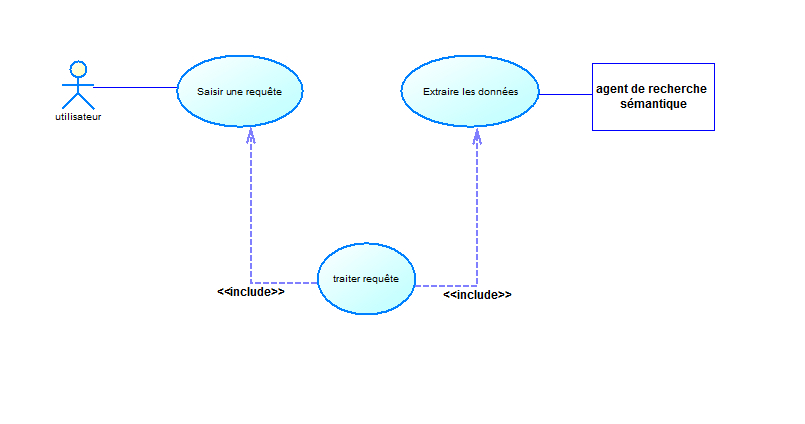
\includegraphics[width=20cm]{cas_utilisation}\\
                    \caption{diagramme des cas d'utilisation}\label{diagramme des cas d'utilisation}
            \end{figure}
        \subsection{Diagramme de séquences de point de vue système}
        Afin de décrire le scénario global de l'application nous avons proposé de construire le diagramme de séquences de point de vue système.\\
        Lorsque l'utilisateur saisit une requête , le système va procéder à son analyse. Deux cas se présentent:\\
        Dans le premier cas la requête contient une erreur de saisie. Donc le système va alors afficher un message d'erreur.\\
        Dans le deuxième  cas la requête est considéré comme valide donc le système procède au traitement nécessaire et retourne le résultat final à l'utilisateur.\\
        \begin{figure}[H]
                    \centering
                    % Requires \usepackage{graphicx}
                    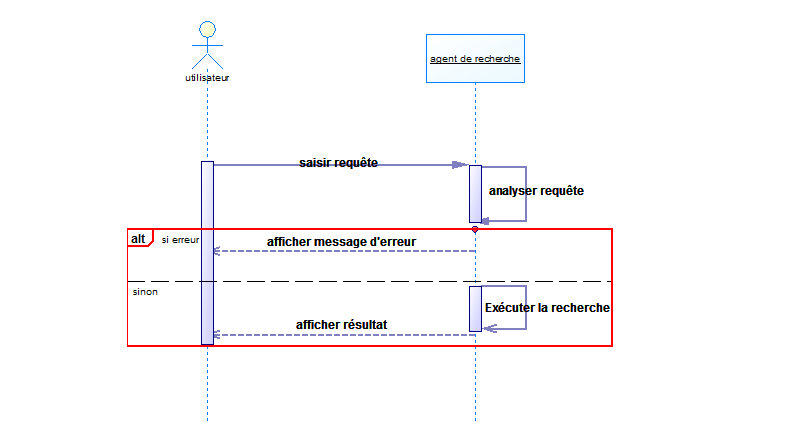
\includegraphics[width=20cm]{diagramme_sequence_system}\\
                    \caption{diagramme de sequences de point de vue systèm}\label{diagramme sequence system}
        \end{figure}
        \subsection{Diagramme de séquences détaillé}
        Suite à la déscription du  scénario général de l'application à travers le diagramme des séquences de point de vue système, on va maintenant décrire le fonctionnement et les interactions entre les différentes entités à l'aide d'un diagramme de séquences détaillé.\\
            \begin{figure}[H]
                    \centering
                    % Requires \usepackage{graphicx}
                    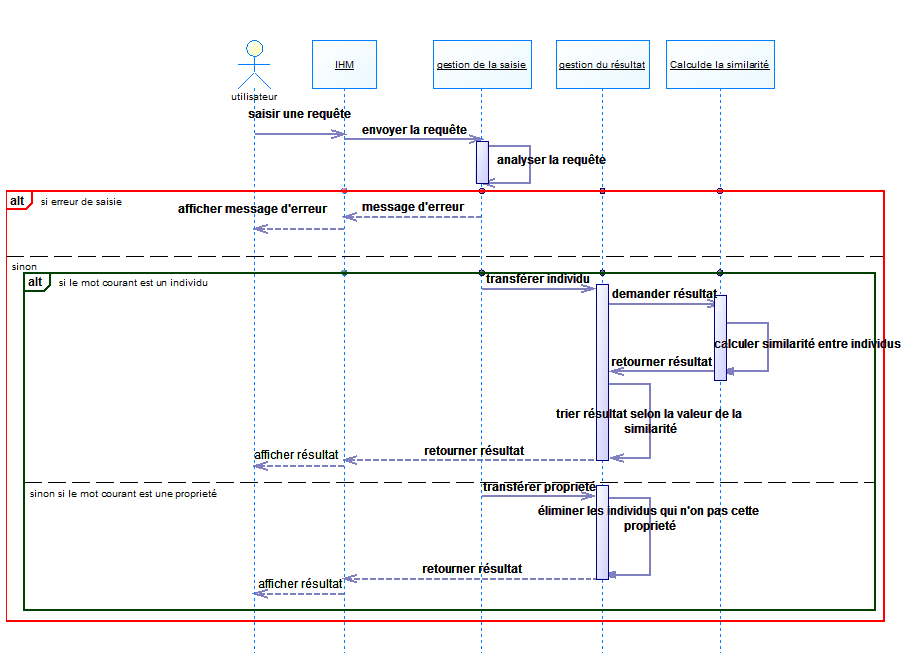
\includegraphics[width=17cm]{diag_sequence_detaille}\\
                    \caption{diagramme de sequences détaillé}\label{diagramme de sequence détaillé}
        \end{figure}
\section{Réalisation et tests}
    Aprés avoir analysé et défni les différentes parties qui constituent notre
    application, nous allons commencer la phase de réalisation et de tests. Celle-ci
    constitue le dernier volet de ce rapport. Elle a pour but d'exposer le travail
    achevé. Nous présenterons donc les différents Module réalisés et nous finissons par des tests.\\
    \subsection{Module de l'extraction des données}
                En se basent sur le diagramme des cas d'utilisation présenté précédemment, le traitement des requêtes ne peut se faire que lorsque le système a bien effecuté l'extraction des données à partir de l'ontologie en gardant les liens de parenté propres aux concepts et aux individus.\\
                Et pour garder ces caractéristiques nous avons  choisi de classer les entités de l'ontologie dans une structure de données arborescente.\\
                L'extraction des données se fait en parcourant le fichier qui décrit l'ontologie ,écrit en langage OWL et le système réagit à chaque ligne de code.\\
                Tout d'abord le système génère l'arborescence de l'ontologie en instanciant les classes ou les concepts et en établissant les liens de parenté entre eux au fur et à mesure du parcours du fichier.
                Ensuite il définit tous les individus de l'ontologie en ajoutant à chacun les  propriétés de types objet ou de type de donnée correspondantes.

    \subsection{Modéle MVC}
        Le modèle MVC est un modèle qui s'applique à la conception de tous les types d'applications qui présentent une interface homme-machine afin de séparer la couche métier de la couche IHM par l'intermédiaire du contrôleur. Chose qui facilite énormément la maintenance des logiciels\\
        Il découpe  l'application en trois couches distinctes:\\
        \begin{itemize}
            \item[\quad $\bullet$]
            Le contrôleur permet d’établir le lien entre la vue et le modèle. C’est le chef d’orchestre de l’application. Il ne fait qu’appeler des méthodes d'implémentation dans le  modèle ou dans la vue.
            \item[\quad $\bullet$]La vue représente l’interface homme-machine. Elle ne fait aucun traitement de données. Sa fonction se résume à la lecture de la requête de l’utilisateur et l’affichage du résultat.
            \item[\quad $\bullet$]C’est la couche métier de l’application : le modèle analyse la requête introduite par l’utilisateur, éffectue le traitement de cette requête en utilisant différents algorithmes performants de recherche selon la similarité.
        \end{itemize}
        \begin{figure}[H]
                    \centering
                    % Requires \usepackage{graphicx}
                    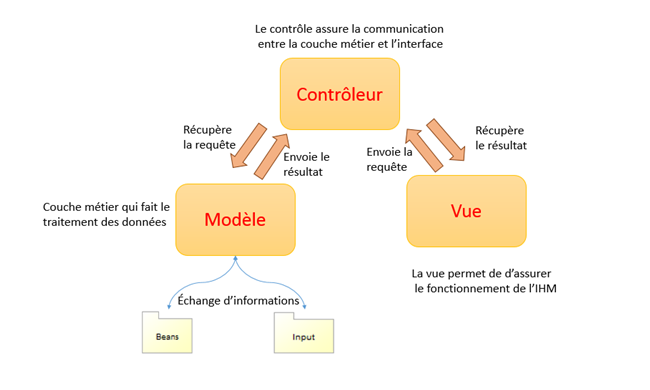
\includegraphics[width=17cm]{mvc}\\
                    \caption{Modéle MVC}\label{Modéle MVC}
        \end{figure}
    \subsection{Tests et validation}
        Tous nos tests dans cette partie seront basés sur un fichier écrit en langage OWL fourni dans l'annexe. La figure suivante générée par Protégé est une représentation graphique simplifiée de l'ontologie. Elle sert à suivre et à vérifier les tests que nous allons implémenter.\\
        \begin{figure}[H]
                    \centering
                    % Requires \usepackage{graphicx}
                    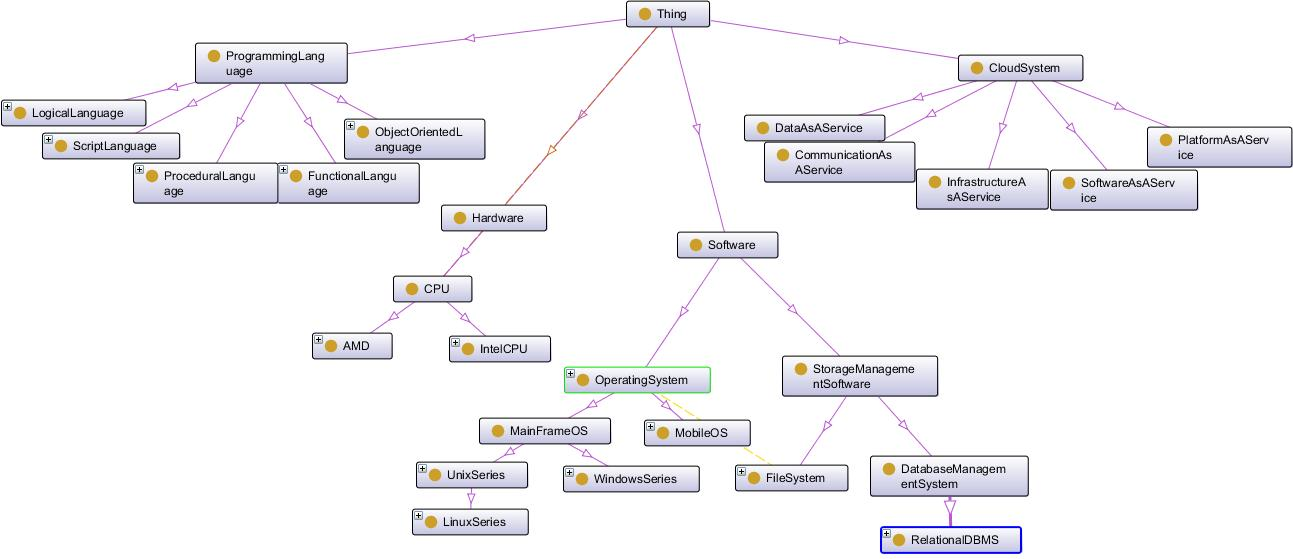
\includegraphics[width=15cm]{cloudle_ontologie}\\
                    \caption{Cloud ontologie}\label{cloud ontologie}
        \end{figure}

        \subsubsection{Extraction des données}
                        Pour tester l'extraction des données on indique quelle ontologie doit-on considérer. Dans notre cas nous avons choisi Cloud.owl. Il suffit d'appeler la méthode qui affiche l'ontologie tout en gardant les liens de parenté.\\
            \begin{figure}[H]
                    \centering
                    % Requires \usepackage{graphicx}
                    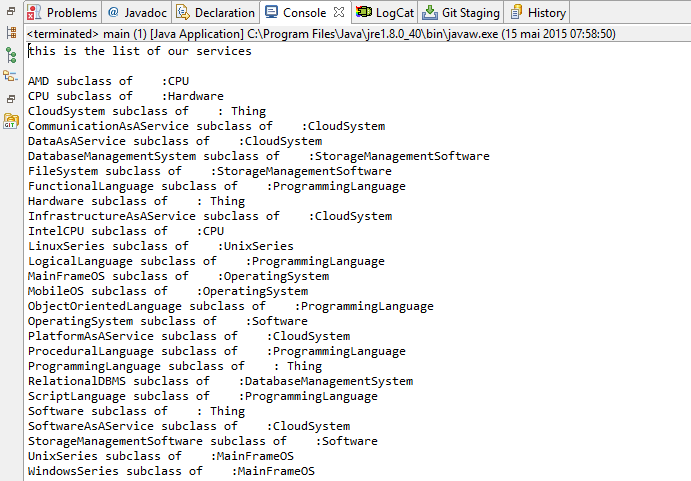
\includegraphics[width=14cm]{imprime_concepts}\\
                    \caption{impr1}\label{impr1}
        \end{figure}
        \subsubsection{Tests des requêtes}
            Lorsque l'utilisateur saisit une requête, deux cas de figure se présentent:\\
            \begin{itemize}
                \item[\quad $\bullet$]Si la requête n'est pas valide, un message d'erreur s'affiche sur l'écran en indiquant l'anomalie rencontrée à travers une boite de dialogue:
                    \begin{figure}[H]
                    \centering
                    % Requires \usepackage{graphicx}
                    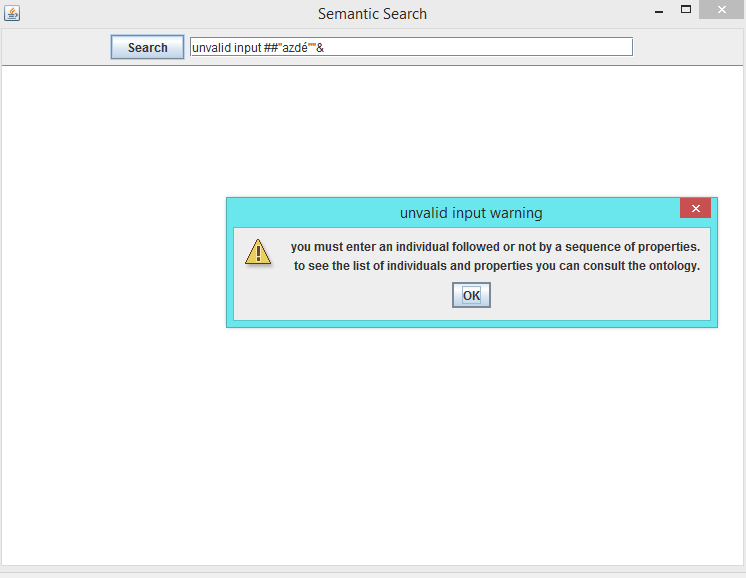
\includegraphics[width=14cm]{impr2}\\
                    \caption{impr2}\label{impr2}
                     \end{figure}
                \item[\quad $\bullet$]Si la requête est valide le résultat s'affiche sur l'écran:
                Soit les trois requêtes suivantes:
                    \begin{figure}[H]
                    \centering
                    % Requires \usepackage{graphicx}
                    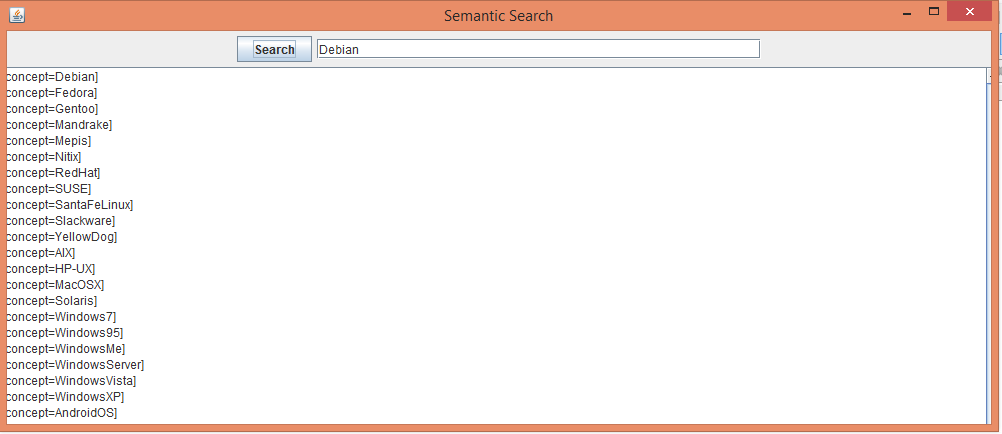
\includegraphics[width=15cm]{imr_debian}\\
                    \caption{imr debian}\label{imr debian}
                    \end{figure}
                     Lorsque l'utilisateur saisie le mot : Debian qui est un individu de l'ontologie de type système d'exploitation le système va afficher les individus classés par ordre de similarité décroissante.

                    \begin{figure}[H]
                    \centering
                    % Requires \usepackage{graphicx}
                    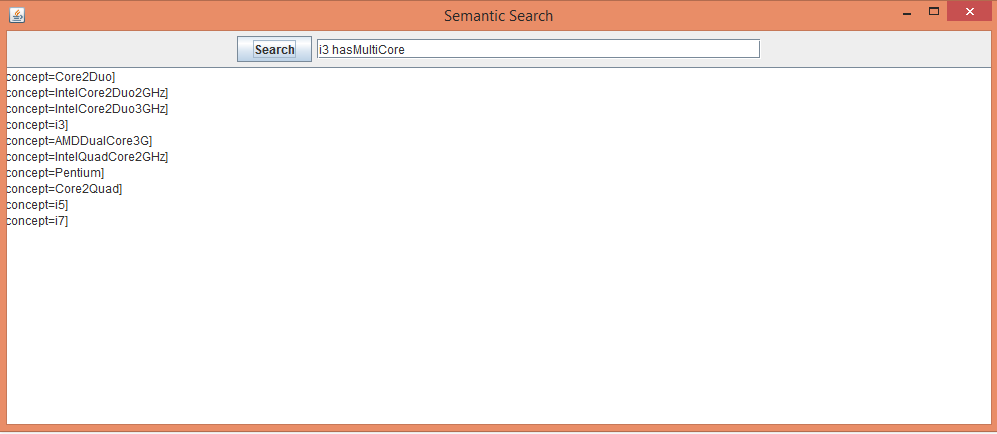
\includegraphics[width=15cm]{imprime_i3_hasMultiCore}\\
                    \caption{imprime i3 hasMultiCore}\label{imprime i3 hasMultiCore}
                    \end{figure}
                      Si l'utilisateur saisit la requête suivante: "i3 hasMultiCore" le système va afficher le résultat par ordre décroissant de la valeur de la similarité en éliminant les individus qui n'ont pas la propriété "hasMultiCore"
                    \begin{figure}[H]
                    \centering
                    % Requires \usepackage{graphicx}
                    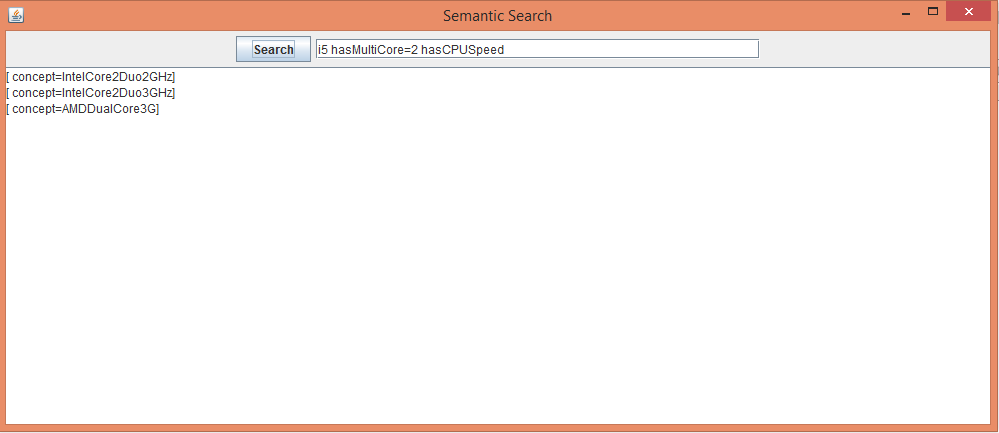
\includegraphics[width=15cm]{imprime_i5}\\
                    \caption{imprime i5 }\label{imprime i5}
                    \end{figure}
                    Lorsque l'utilisateur saisit : "i5 hasMultiCore=2 hasCPUSpeed" le système va chercher les individus similaires à i5 ,il va ensuite éliminer les entités qui n'ont pas la propriété hasMultiCore avec la valeur 2 et hasCPUSpeed et va trier le résultat par ordre décroissant de la similarité.

            \end{itemize}



\section{Conclusion}
    Dans ce chapitre nous avons introduit les outils utilisés pour l'implémentation de notre application. Suite à çela nous avons proposé la conception adéquate à ce système de recherche et nous avons terminé par la partie réalisation et tests.\\

















\addcontentsline{toc}{chapter}{Conclusion et Perspectives}
\chapter*{Conclusion et Perspectives}

Notre projet se situe dans le cadre de l'optimisation du processus de recherche des services Cloud à travers la manipulation des ontologies du Cloud et le calcul de similarité.
C'est dans cet esprit là que nous allons dresser un bilan de notre travail et présenter quelques perspectives future.\\

\textbf{Bilan et contributions}

En vue de réaliser l'objectif qu'on s'est imposé , nous avons divisé la charge de travail en plusieurs étapes.
Nous avons donc procédé à la collecte de documents , articles , théses traitant le sujet ainsi que les projets existants.
Nous nous sommes donc principalement interessé au fonctionnement du moteur de recherche de services Cloud : "Cloudle " du fait qu'il se base sur la consultation et la manipulation d'une antologie du web.
Cependant même si "Cloudle" traite la similarité de concepts , il considére les propriétés existantes tel que le stockage mémoire ,la vitesse du processeur comme étant des concepts apparentières ce qui rend la recherche moins performante qu'elle aurait dû être.
Alors que la recherche avec "Cloudle" repose sur le calcul de similarité entre concepts et sur le raisonnement équivalent et numérique entre les concepts , nous avons décidé de partir sur une approche partiellement différente de celle utilisée par "Cloudle".
En effet , en plus d'avoir recours à la consultation d'une ontologie du Cloud et du calcul de similarité de concepts , notre approche consiste dans le développement d'un algorithme de recherche qui met au point l'utilisation des similarités des propriétés objet et type de données pour ajouter à la précision et l'efficacité de la recherche pour ainsi obtenir non seulement un procédé de recherche dont les résultats sont précis mais répondent à l'attente des utilisateurs.

Ce projet nous a bénéficier tant sur le plan théorique que pratique.En effet , il nous a permit de nous ouvrir sur de tout nouveaux domaines dont nous ignorions tout qui sont le Cloud Computing et Le web sémantique.
De plus , nous avons pû renforcer notre maîtrise du language de programmation Java avec lequel nous avons developpé notre application.\\

\textbf{Perspectives de recherche}
L'algorithme que nous avons developpé , a été testé à plusieurs reprises sur de diverses ontologies et a donné des résultats très satistfaisant .
Cependant, nous n'avons pu étudier que les cas d'ontologies à la structure assez simple , ceci dû à la fois au manque de ressources et de temps à notre disposition.
Cela n'empêche que nous désirons essayer notre algorithme sur des ontologies aux structures beaucoup plus complexes pour comparer les résultats obtenus lors du passage à l'échelle et potentiellement adapter notre travail à l'utilisation dans le marché actuel. 
%--------------------------------------
%\addcontentsline{toc}{chapter}{Bibliographie}

\addcontentsline{toc}{chapter}{Bibliographie}
\bibliographystyle{alpha}
\nocite{*}
%\bibliography{bib}
\addcontentsline{toc}{chapter}{Annexe}
%\chapter*{Annexe A : Charge utilisée pour l’expérimentation de notre stratégie de sélection des IJB}
\markboth{Annexe}{}
\textbf{Q1} - select sum(lo\_extendedprice*lo\_discount) as revenue from lineorder, dates where lo\_orderdate = d\_datekey and d\_year = 1993 and lo\_discount >= 1 and lo\_discount <= 3 and lo\_quantity < 25 \\

\textbf{Q2} - select count(*) from lineorder, dates where lo\_orderdate = d\_datekey and d\_year = 1993 and lo\_discount >= 1 and lo\_discount <= 3 and lo\_quantity < 25 \\

\textbf{Q3} - select sum(lo\_extendedprice*lo\_discount) as revenue from lineorder, dates where lo\_orderdate = d\_datekey and d\_year = 1993 \\

\textbf{Q4} - select count(*) from lineorder, dates where lo\_orderdate = d\_datekey and d\_year = 1993 \\

\textbf{Q5} - select sum(lo\_revenue), d\_year from lineorder, dates, part, supplier where lo\_orderdate = d\_datekey and lo\_partkey = p\_partkey and lo\_suppkey = s\_suppkey and p\_brand = 'MFGR\#2221' and s\_region = 'ASIA' group by d\_year order by d\_year \\

\textbf{Q6 }- select sum(lo\_revenue) from lineorder, part where lo\_partkey = p\_partkey and p\_brand = 'MFGR\#2221' \\

\textbf{Q7} - select avg(lo\_revenue), d\_year from lineorder, dates, part, supplier where lo\_orderdate = d\_datekey and lo\_partkey = p\_partkey and lo\_suppkey = s\_suppkey and p\_brand = 'MFGR\#2221' and s\_region = 'ASIA' group by d\_year order by d\_year \\

\textbf{Q8} - select sum(lo\_revenue), d\_year from lineorder, dates, part, supplier where lo\_orderdate = d\_datekey and lo\_partkey = p\_partkey and lo\_suppkey = s\_suppkey and p\_brand = 'MFGR\#2221' and s\_region = 'EUROPE' group by d\_year, p\_brand order by d\_year, p\_brand \\

\textbf{Q9} - select sum(lo\_revenue) from lineorder, part, supplier where lo\_partkey = p\_partkey and lo\_suppkey = s\_suppkey and p\_brand = 'MFGR\#2221' and s\_region = 'EUROPE' \\

\textbf{Q10} - select count(*), d\_year from lineorder, dates, part, supplier where lo\_orderdate = d\_datekey and lo\_partkey = p\_partkey and lo\_suppkey = s\_suppkey and p\_brand = 'MFGR\#2221' and s\_region = 'EUROPE' group by d\_year order by d\_year \\

\textbf{Q11} - select c\_nation, s\_nation, d\_year, sum(lo\_revenue) as revenue from lineorder,customer,  supplier, dates where lo\_custkey = c\_custkey and lo\_suppkey = s\_suppkey and lo\_orderdate = d\_datekey and c\_region = 'ASIA' and s\_region = 'ASIA' and d\_year >= 1992 and d\_year <= 1997 group by c\_nation, s\_nation, d\_year order by d\_year asc, revenue desc \\

\textbf{Q12 }- select s\_nation, sum(lo\_revenue) as revenue from lineorder, supplier where lo\_suppkey = s\_suppkey and s\_region = 'ASIA' group by s\_nation order by revenue desc \\

\textbf{Q13} - select s\_nation, count(*) as revenue from lineorder, supplier where lo\_suppkey = s\_suppkey and s\_region = 'ASIA' group by s\_nation order by revenue desc \\

\textbf{Q14} - select s\_nation, d\_year, sum(lo\_revenue) as revenue from lineorder, supplier, dates where lo\_suppkey = s\_suppkey and lo\_orderdate = d\_datekey and s\_region = 'ASIA' and d\_year >= 1992 and d\_year <= 1997 group by s\_nation, d\_year order by d\_year asc, revenue desc \\

\textbf{Q15} - select c\_nation, s\_nation, d\_year, avg(lo\_revenue) as avg\_revenue from lineorder,customer,  supplier, dates where lo\_custkey = c\_custkey and lo\_suppkey = s\_suppkey and lo\_orderdate = d\_datekey and c\_region = 'ASIA' and s\_region = 'ASIA' and d\_year >= 1992 and d\_year <= 1997 group by c\_nation, s\_nation, d\_year order by d\_year asc, avg\_revenue desc \\

\textbf{Q16} - select c\_nation, s\_nation, d\_year, count(*) from lineorder,customer,  supplier, dates where lo\_custkey = c\_custkey and lo\_suppkey = s\_suppkey and lo\_orderdate = d\_datekey and c\_region = 'ASIA' and s\_region = 'ASIA' and d\_year >= 1992 and d\_year <= 1997 group by c\_nation, s\_nation, d\_year order by d\_year asc \\

\textbf{Q17} - select c\_city, s\_city, d\_year, sum(lo\_revenue) as revenue from lineorder,customer,  supplier, dates where lo\_custkey = c\_custkey and lo\_suppkey = s\_suppkey and lo\_orderdate = d\_datekey and c\_nation = 'UNITED STATES' and s\_nation = 'UNITED STATES' and d\_year >= 1992 and d\_year <= 1997 group by c\_city, s\_city, d\_year order by d\_year asc, revenue desc \\

\textbf{Q18} - select s\_city, sum(lo\_revenue) as revenue from lineorder, supplier where lo\_suppkey = s\_suppkey and s\_nation = 'UNITED STATES' group by s\_city order by revenue desc \\

\textbf{Q19} - select s\_city, avg(lo\_revenue) as avg\_revenue from lineorder, supplier where lo\_suppkey = s\_suppkey and s\_nation = 'UNITED STATES' group by s\_city order by avg\_revenue desc \\

\textbf{Q20} - select c\_city, s\_city, count(*) from lineorder,customer,  supplier where lo\_custkey = c\_custkey and lo\_suppkey = s\_suppkey and c\_nation = 'UNITED STATES' and s\_nation = 'UNITED STATES' group by c\_city, s\_city \\

\textbf{Q21} - select c\_city, s\_city, d\_year, avg(lo\_revenue) as avg\_revenue from  lineorder,customer, supplier, dates where lo\_custkey = c\_custkey and lo\_suppkey = s\_suppkey and lo\_orderdate = d\_datekey and c\_nation = 'UNITED STATES' and s\_nation = 'UNITED STATES' and d\_year >= 1992 and d\_year <= 1997 group by c\_city, s\_city, d\_year order by d\_year asc, avg\_revenue desc \\

\textbf{Q22} - select c\_city, s\_city, d\_year, count(*) from lineorder,customer,  supplier, dates where lo\_custkey = c\_custkey and lo\_suppkey = s\_suppkey and lo\_orderdate = d\_datekey and c\_nation = 'UNITED STATES' and s\_nation = 'UNITED STATES' and d\_year >= 1992 and d\_year <= 1997 group by c\_city, s\_city, d\_year order by d\_year asc \\

\textbf{Q23 }- select d\_year, s\_nation, p\_category, sum(lo\_revenue - lo\_supplycost) as profit from lineorder,dates, customer, supplier, part  where lo\_custkey = c\_custkey and lo\_suppkey = s\_suppkey and lo\_partkey = p\_partkey and lo\_orderdate = d\_datekey and c\_region = 'AMERICA' and s\_region = 'AMERICA' and (d\_year = 1997 or d\_year = 1998) and (p\_mfgr = 'MFGR\#1' or p\_mfgr = 'MFGR\#2') group by d\_year, s\_nation, p\_category order by d\_year, s\_nation, p\_category \\

\textbf{Q24} - select d\_year, s\_nation, p\_category, sum(lo\_revenue - lo\_supplycost) as profit from lineorder, dates, supplier, part  where lo\_suppkey = s\_suppkey and lo\_partkey = p\_partkey and lo\_orderdate = d\_datekey and s\_region = 'AMERICA' and (d\_year = 1997 or d\_year = 1998) and (p\_mfgr = 'MFGR\#1' or p\_mfgr = 'MFGR\#2') group by d\_year, s\_nation, p\_category order by d\_year, s\_nation, p\_category \\

\textbf{Q25} - select d\_year, s\_nation, p\_category, avg(lo\_revenue - lo\_supplycost) as avg\_profit from lineorder, dates, customer, supplier, part   where lo\_custkey = c\_custkey and lo\_suppkey = s\_suppkey and lo\_partkey = p\_partkey and lo\_orderdate = d\_datekey and c\_region = 'AMERICA' and s\_region = 'AMERICA' and (d\_year = 1997 or d\_year = 1998) and (p\_mfgr = 'MFGR\#1' or p\_mfgr = 'MFGR\#2') group by d\_year, s\_nation, p\_category order by d\_year, s\_nation, p\_category \\

\textbf{Q26} - select d\_year, s\_nation, p\_category, count(*) from lineorder, dates, customer, supplier, part  where lo\_custkey = c\_custkey and lo\_suppkey = s\_suppkey and lo\_partkey = p\_partkey and lo\_orderdate = d\_datekey and c\_region = 'AMERICA' and s\_region = 'AMERICA' and (d\_year = 1997 or d\_year = 1998) and (p\_mfgr = 'MFGR\#1' or p\_mfgr = 'MFGR\#2') group by d\_year, s\_nation, p\_category order by d\_year, s\_nation, p\_category \\

\textbf{Q27} - select d\_year, s\_nation, count(*) from  lineorder,dates, supplier  where lo\_suppkey = s\_suppkey and lo\_orderdate = d\_datekey and s\_region = 'AMERICA' and (d\_year = 1997 or d\_year = 1998) group by d\_year, s\_nation order by d\_year, s\_nation \\

\textbf{Q28} - select s\_nation, count(*) from lineorder,supplier   where lo\_suppkey = s\_suppkey and s\_region = 'AMERICA' group by s\_nation order by s\_nation \\

\textbf{Q29} - select d\_year, s\_nation, sum(lo\_revenue) as revenue from lineorder,dates, supplier   where lo\_suppkey = s\_suppkey and lo\_orderdate = d\_datekey and s\_region = 'AMERICA' and (d\_year = 1997 or d\_year = 1998) group by d\_year, s\_nation order by d\_year, s\_nation \\

\textbf{Q30} - select sum(lo\_revenue), p\_brand from lineorder, part, supplier where lo\_partkey = p\_partkey and lo\_suppkey = s\_suppkey and p\_brand = 'MFGR\#2221' and s\_region = 'ASIA' group by p\_brand order by p\_brand



\end{document} 